\section{Performance and scalability}
\label{performance}

Performance evaluation of the automated subject classification component is
treated in section \ref{autoclasseval}.

\subsection{Speed}

Performance in terms of number of URLs treated per minute is of course
highly dependent on a number of circumstances like network load,
capacity of the machine, the selection of URLs to crawl, configuration
details, number of crawlers used, etc.
In general, within rather wide limits, you could expect the Combine
system to handle up to 200 URLs per
minute. By ``handle'' we mean everything from scheduling of URLs, fetching
 pages over the network, parsing the page,
automated subject classification, recycling of new links, to storing the structured record in
a relational database. This holds for small simple crawls starting
from scratch to large complicated topic specific crawls with millions
of records.

\begin{figure}[htb]
\begin{center}
 \includegraphics[height=0.4\textheight]{CrawlerSpeed.ps}
\end{center}
\caption{Combine crawler performance, using no focus and configuration optimized for speed.}
\label{crawlspeed}
\end{figure}

The prime way of increasing performance is to use more than one
crawler for a job. This is handled by the \verb+--harvesters+ switch
used together with the {\tt combineCtrl start} command for example
\verb+combineCtrl --jobname MyCrawl --harvesters 5 start+
will start 5 crawlers working together on the job 'MyCrawl'. The
effect of using more than one crawler on crawling speed is illustrated
in figure \ref{crawlspeed} and the resulting speedup is shown in table \ref{speedup}.

\begin{table}[h]
\begin{center}
\begin{tabular}{|l|c|c|c|c|c|c|}
\hline
{\bf No of crawlers}& 1& 2& 5& 10& 15& 20\\ \hline
{\bf Speedup}& 1& 2.0& 4.8& 8.2& 9.8& 11.0\\ \hline
\end{tabular}
\end{center}
\caption{Speedup of crawling vs number of crawlers}
\label{speedup}
\end{table}

Configuration also has an effect on performance. In Figure
\ref{config} performance improvements based on configuration changes are shown. The choice of
algorithm for automated classification turns out to have biggest
influence on performance, where \hyperref{algorithm 2}{algorithm 2 -- section }{ --}{pos} ({\tt classifyPlugIn = Combine::PosCheck\_record} -- Pos in Figure \ref{config}) is much
faster than \hyperref{algorithm 1}{algorithm 1 -- section }{ --}{std} ({\tt classifyPlugIn = Combine::Check\_record} -- Std in Figure \ref{config}).
Configuration optimization consisted of not using
Tidy to clean HTML ({\tt useTidy = 0}) and not storing the original
page in the database ({\tt saveHTML = 0}).
 Tweaking of other configuration variables (like disabling logging
to the MySQL database {\tt Loglev = 0}) also has an effect
on performance but to a lesser degree.

\begin{figure}[htb]
\begin{center}
 \includegraphics[height=0.4\textheight]{Config.ps}
\end{center}
\caption{Effect of configuration changes on focused crawler performance, using 10 crawlers and a topic definition with 2512 terms.}
\label{config}
\end{figure}

\subsection{Space}

Storing structured records including the original document takes
quite a lot of disk space. On average 25 kB per record is
used by MySQL. This includes the administrative overhead needed
for the operation of the crawler. A database with 100~000 records
needs at least 2.5 GB on disk. Deciding not to store the original
page in the database ({\tt saveHTML = 0}) gives considerable space
savings. On average 8 kB per is used without the original HTML.

%MySQL DB   Recs  Size kB   PerRec kB
%searcheng 919466 21926944  23.8
%B2        518604 12832348  24.7
%CP        202519  6002156  29.6
%algebra    80589  3445140  42.7
%
%Export format combine
%DB         recs  size B      PerRec kB Time (min)
%algebra    80589  2585870648 32        118
%B2        518604 14214575712 27       1415
%
%Export format alvis
%B2        518604 21742558821 42       3413
%
%Export format dc
%B2        518604   813749518        1343m33.391s
%

Exporting records in the ALVIS XML format further increases size
to 42 kB per record. Using the slight less redundant XML-format
{\tt combine} uses 27 kB per record. Thus 100~000 records will generate
a file of size 3 to 4 GB. The really compact Dublin Core format ({\tt dc}) generates 0.65 kB per record.

\subsection{Crawling strategy}

In \cite{Rafael06} four different crawling strategies are studied:
\begin{description}
\item[BreadthFirst]
The simplest strategy for crawling. 
It does not utilize heuristics in deciding which URL to visit next. 
It uses the frontier as a FIFO queue, crawling links in the order in which 
they are encountered.

\item[BestFirst]
The basic idea is that given a frontier of URLs, the best URL
according to some estimation criterion is selected for crawling,
using the frontier as a priority queue.
In this implementation, the URL selection process is guided by 
the topic score of the source page as calculated by Combine.

\item[PageRank] The same as Best-First but ordered by PageRank calculated
from the pages crawled so far.

\item[BreadthFirstTime]
A version of BreadthFirst.
It is based on the idea of not accessing the same server during 
a certain period of time in order not to overload servers.
Thus, a page is fetched if and only if 
a certain time threshold is exceeded 
since the last access to the server of that page.

\end{description}

Results from a simulated crawl (figure \ref{crawlstrategy} from \cite{Rafael06}) show that
at first PageRank performs best but BreadthFirstTime (which is used in Combine) prevails
in the long run, although differences are small.

\begin{figure}[htbp]
\begin{center}
%  \includegraphics[width=100mm, height=75mm]{crawl.jpg}
  \includegraphics[width=140mm, height=90mm]{crawl.ps}
  \caption{Total number of relevant pages visited}
 \label{crawlstrategy}
\end{center}
\end{figure}
